\documentclass{article}
\usepackage{caption}
\usepackage{graphicx}
\usepackage[margin=1.5in]{geometry}
\usepackage{listings}

\newcommand\email{andredbsc@gmail.com}
\newcommand\discord{dbsc\#3718}

\title{ZK University \\[4pt] \normalsize\textsc{Week 3 Submission}}
\author{André Dal Bosco \\ \small{\email \quad \discord}}

\begin{document}
\maketitle

\subsection*{Circom in games}
\begin{itemize}
    \item In \texttt{Part1/contracts/circuits/}, \texttt{hitandblow.circom} is a circuit that implements the simple Hit \& Blow (aka Mastermind) game adapted from here and here. What have the authors done in their implementations to protect them from brute-force attacks? \par First we have to analyse what exactly this circuit is aiming to accomplish. The one way an attacker could brute-force his way to the solution is just calculating all the possible public hashes derived from code combinations and test them, until one actually matches the hash derived from the private solution. But the addition of salt to the hash formula actually makes this impossible, since the number of possibilities is now much bigger (the salt could be a small or a very big number which introduces a lot of new possibilities).
    \item In \texttt{test/mastermind-test.js}, write unit tests to test the functionality of your circuit from Q2. Attach a screenshot of your unit tests passing.
    \begin{figure}[h]
        \centering
        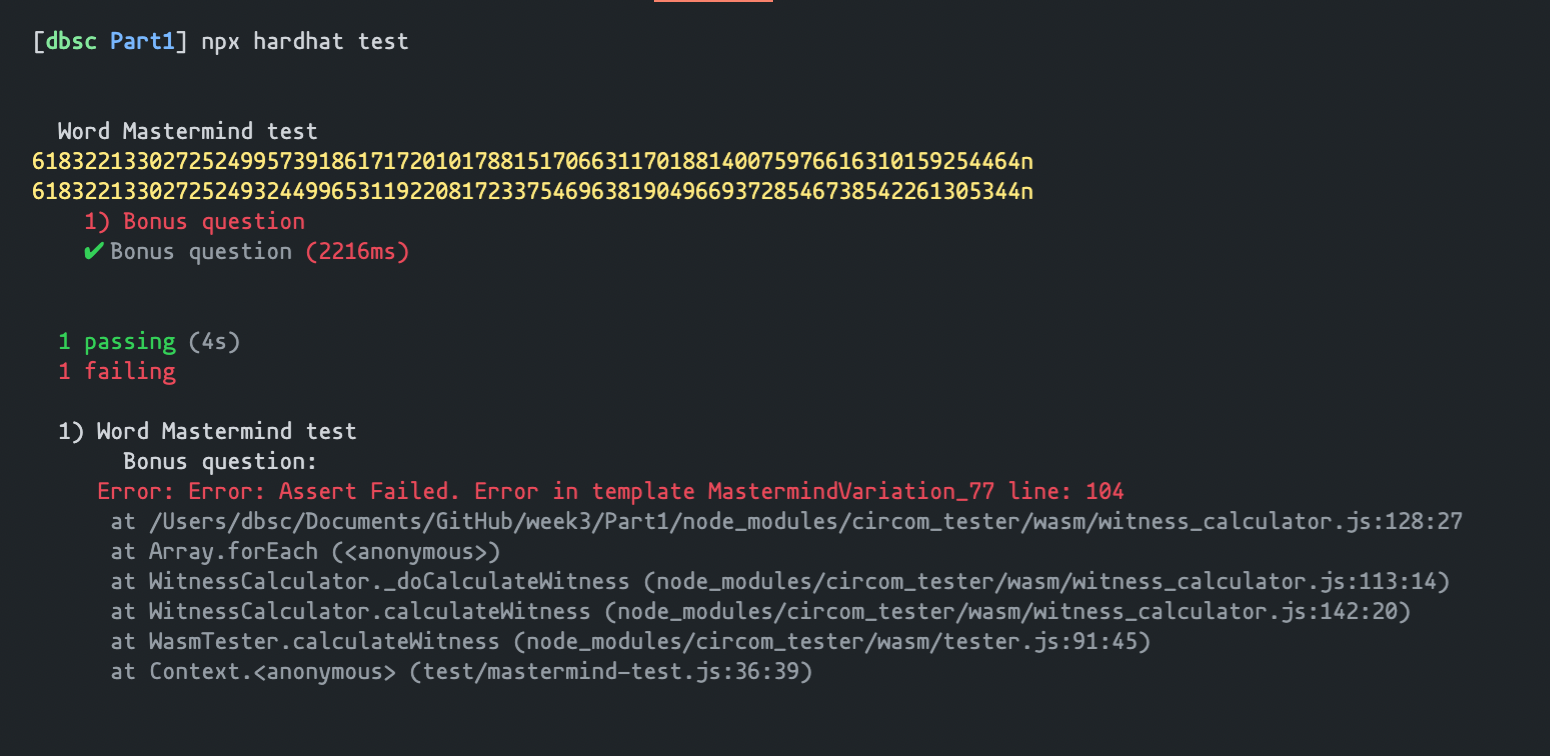
\includegraphics[width=0.7\textwidth]{test.png}
        \caption*{Tests for Word Mastermind.}
    \end{figure}

    The reason why it failed is that the two yellow numbers, one representing the public hash of the solution, and the other derived from the private solution and salt, differ on some digits, and I'm not sure yet why that is.
    \item There are many games that could benefit from the privacy ZK offers and can be protected from brute-force attacks using the same technique. Previous graduates have built the classic Hangman and Battleship, as well as some original games such as zkAutoChess and zkWitches for their final projects. Suggest / Design a game and explain (1) how it is played, (2) how it can benefit from ZK, (3) how it can be implemented with ZK, (4) how it is protected from brute-force attacks. \par Chase game: a two player game where there's a chaser, and a fugitive. The fugitive spans 15 units from the chaser, and must naturally run away from the chaser. The chaser can move anywhere between 1 and 4 units of distance each round, whereas the fugitive can run 1 unit of distance each round, and 2 additional bonus units each three rounds. On the first round, the chaser moves, and on the second round, the fugitive gets to move, and so on. The game happens on a square lattice world. The position of the fugitive is not revealed, whereas the position of the chaser is public. The game ends when both players meet. The chaser must guide himself using arrows that can point horizontally, vertically, or diagonally. The fugitive produces a zero knowledge proof to assert the validity of the helper arrow without surrendering his true position. To implement the circuit, we can think of the arrow direction as a public input ranging from 0 to 7, the chaser position as a public input, and the fugitive position as a private input. We prove that the arrow is pointing in the correct direction with simple calculations. If we don't add salt to the mix, the chaser can very easily break the fugitive position (just follow the arrow until it turns direction, meaning the proof is now invalid, which indicates the fugitive's position).
\end{itemize}

\subsection*{Anti-collusion and Fairness}
\begin{itemize}
    \item Summarize how MACI works in 2-4 sentences of simple English. \par MACI basically allows people to vote but change it later if needed. So if A writes down his vote and locks in a box to which only C has a key. Although B may have forced A to vote in a certain way, A has the ability to go and change it later, so B cannot be sure if A has been effectively coerced.
    \item What kind of collusion(s) does MACI solve? \par It solves collusions where there's a bribe, because the seller can change his vote without any drawbacks.
    \item What kind of collusion(s) or attack(s) does MACI not solve? \par If a big enough group of people come together in a malicious way, they can possibly overpower the vote.
    \item Explain in 1-3 sentences why, in computing VDFs, having many computers operating in parallel won't help you to find the solution more quickly. \par The major bottleneck part of the computation is sequential, so introducing parallelism won't improve things that much.
    \item Think of and explain an upgraded design of ZK Blind Auction that eliminates the need for a centralized server while maintaining the privacy of the bid value, i.e. only the bidder knows their own bid value. Assume that a multi-phase design is possible and we can somehow incentivize the bidders to come back and submit multiple proofs/transactions. \par The bids can be submitted in an encrypted form to the blockchain, for example using the own bidder's private key. Then, this private key can be used as private input to find out the winning bid, without revealing the bids themselves. Of course, this doesn't sound totally safe, I'm currently thinking of alternative ways to do it.
    \item One way to ensure the bidders will come back to reveal their bid values and/or claim the auction item is to make them deposit at the time of bidding. Propose a scheme so that bidders can pre-deposit some tokens at the time of bidding without revealing their bidding value. (If they deposit their bid value on a blockchain, then it will be known to the public.) \par The simplest way I see to solve this, is to just setup a standard stake quantity at the start of the auction, regardless of the bidding value the bidder chooses.
\end{itemize}
\begin{figure}[h]
    \centering
    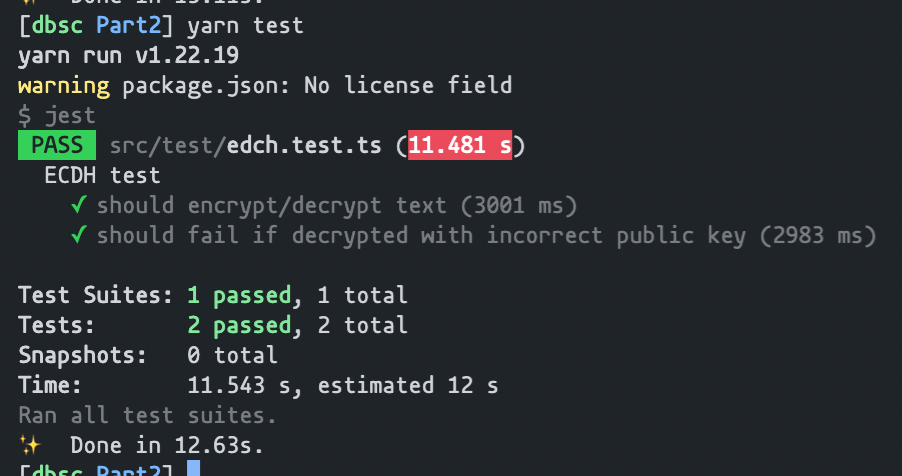
\includegraphics[width=0.7\textwidth]{test2.png}
    \caption*{Tests verifying that Part2/src/index.ts was correctly implemented.}
\end{figure}
\subsection*{Time to start thinking about your final project!}
\begin{itemize}
    \item Suppose you are building the auction application from Part 2 Q4.1 and the circuit is already built for you. Write down an implementation plan, including what other components you will need to build, the order in which you will build your components, as well as what frameworks/tools you will use. \par We modify the initial circuit so that it accepts private keys as private input and the bids' hashes as public input. We instantiate the template as a component. Additionally, I'd use hardhat for testing and deploying.
    \item Suggest three candidate ideas for your final project. Explain (1) the problem tackled, (2) a design overview, and (3) obstacles anticipated in approx. 200 words for each idea. \begin{itemize}
    \item Chase Game \par The game's mechanics were explained shortly above. This game can be achieved without use of blockchain, but then, players will be able to easily cheat if there's not a centralized server (which we don't want), since data would be shared. A zero knowledge proof can be implemented so that the fugitive can prove he's in the direction showed to the chaser without surrendering any other informations, effectively denying any possibility of cheating. It is important to add some salt to the position of the fugitive so it's not easily breakable by brute force.
    \item An app where people are able to send messages to other addresses anonymously. Whoever sends the first message initializes a chat which can later be accessed in some way, maybe with the use of a token, so that the conversation may continue. The sender identitity will be verified using a zero knowledge proof. At first I'm thinking about proving that the sender has the given access token without surrendering any information about the given token. I do not know how exactly I'm gonna design the messasing part of the app, so I'll be looking at other applications that do this and see what I can learn.
    \end{itemize}
\end{itemize}
\end{document}
